\section{可复现性与审计细节}

\subsection{工件账本}
\label{app:ledger}

机器可读账本由发布的账本脚本与重算脚本生成。它记录论文所引每一次运行的源摘要、数据集与逐题 JSONL SHA-256 值，并在论文写作前重新生成、与脚本输出逐字节比对。当前账本覆盖 MemoryAgentBench 各轨道（两代引擎 $\times$ 三条答案路径、commit 455306d 处的官方评分器、一致的 \texttt{entity2id} 指纹）、LongMemEval 整批对话写入后的配对运行与 500 题运行、LoCoMo-1986/1540 及 K3 作答诊断、LoCoMo-Plus-401 \citep{li-etal-2026-locomo}、X7 通道诊断、源扩展诊断、修复后的预算前沿重放、MEME、BigCodeBench \citep{zhuo2024bigcodebench} 与 ALFWorld \citep{shridhar2021alfworld}。每次运行的清单记录数据集与提示词来源、模型标识符、工具观测、证据 ID、延迟、退出状态与代码/运行时哈希；未通过完整性检查的结果与负面结果均予保留而非丢弃。账本生成与重算脚本随发布的补充材料一同提供，因此该链条可端到端重建。

发布的补充材料包含重建每张表所需的机器可读清单、逐题分数、提示词与运行时哈希。论文在每个结果旁报告数据集、模型、评审、子集与完整性状态，使比较保持可审计，同时不暴露机器特定的存储位置。

\begin{figure*}[t]
  \centering
  
\includegraphics[width=\textwidth]{figures/fig1_architecture.pdf}
  \caption{Deep-Dream 的文档优先时序概念图谱。多份文档保留各自的会话片段，并通过共享的概念族与关系边连接。选中一个族会暴露其按观测时间排列的版本链，以及每次修订的精确源跨度；不确定的匹配可以先保持分离，等到后续内容与关系上下文到达时再收敛。}
  \label{fig:architecture}
\end{figure*}

\begin{figure*}[t]
  \centering
  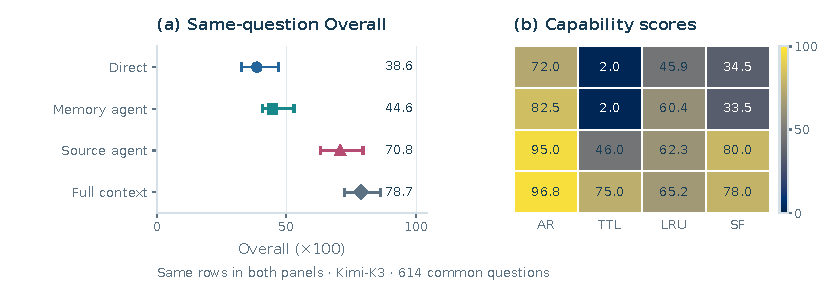
\includegraphics[width=\textwidth]{figures/figA_alignment.pdf}
  \caption{同模型完整上下文参照覆盖的 $n{=}614$ 题上的同题对齐（Kimi-K3 作答；官方宏平均评分器）。（a）带边缘 95\% bootstrap 区间的 Overall 分数；原文读取方式低于参照 $7.9$ 个百分点 [95\% CI $-11.9$, $-3.9$]。（b）域画像：参照的领先集中在 TTL，而原文读取方式在 AR、LRU、SF 上与参照持平或反超。}
  \label{fig:alignment}
\end{figure*}

\begin{figure*}[t]
  \centering
  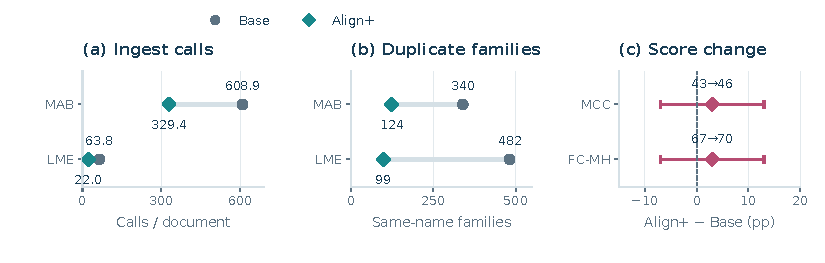
\includegraphics[width=\textwidth]{figures/figB_alignment_outcomes.pdf}
  \caption{捆绑的 Base$\to$Align+ 修订的配对构建诊断。（a）入库调用与同名重复实体族在记录在案的 MAB 与 LongMemEval 交集上下降。（b）配对的 MCC 与 FC-MH 切片各上升 3 个百分点；区间保留，因为这是捆绑比较而非组件消融。}
  \label{fig:alignment-outcomes}
\end{figure*}

\begin{table*}[t]
\centering
\small
\setlength{\tabcolsep}{3.5pt}
\begin{tabular}{@{}p{0.15\textwidth}p{0.23\textwidth}p{0.25\textwidth}p{0.30\textwidth}@{}}
\toprule
\textbf{属性} & \textbf{直接检索} & \textbf{工具辅助读取} & \textbf{原文读取} \\
\midrule
源访问 & top-$k$ 跨度 & 派生记录 & 逐字源文件 \\
工具 & 无 & 记忆工具 & 读取、grep、脚本 \\
答题模型 & 独立 & 独立 & 带验证的智能体 \\
循环 & 无 & 多次只读调用 & 多次读取并核对 \\
每题成本 & \DirectRetrievalCost & \MemoryToolCost & \SourceGroundedCost \\
\bottomrule
\end{tabular}
\caption{三种读取方式的差异。三条路径共享冻结库、问题流、Kimi-K3 与官方评分器。}
\label{tab:answer-path-differences}
\end{table*}

\begin{figure*}[t]
  \centering
  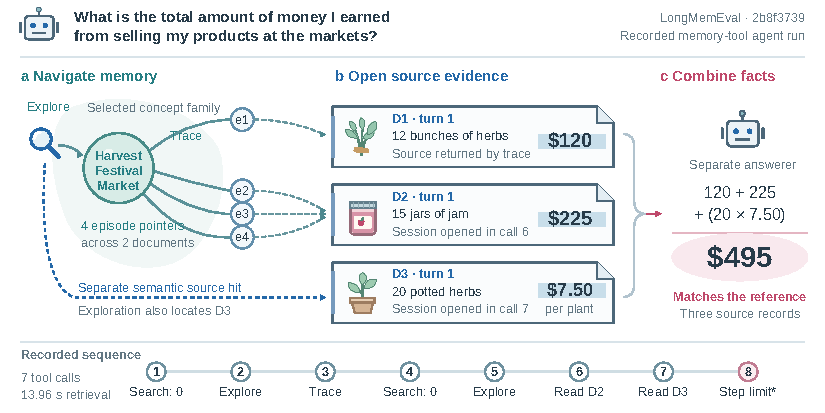
\includegraphics[width=\textwidth]{figures/fig4_agent_trace.pdf}
  \caption{一条实测 LongMemEval 轨迹（问题 \texttt{2b8f3739}）：概念追踪暴露出跨两份文档的四个会话片段指针，另一次语义命中定位到第三条销售记录。七次成功调用耗时 13.96\,s；第 8 步在一次格式错误的响应后达到上限，随后一个独立的答题模型算出 $120+225+(20\times7.5)=495$。}
  \label{fig:agent-trace}
\end{figure*}

\begin{table*}[t]
\centering
\small
\setlength{\tabcolsep}{2.5pt}
\renewcommand{\arraystretch}{1.16}
\begin{tabular*}{\textwidth}{@{\extracolsep{\fill}}p{0.04\textwidth}p{0.25\textwidth}p{0.65\textwidth}@{}}
\toprule
\textbf{RQ} & \textbf{记忆能力} & \textbf{基准与可观测预测} \\
\midrule
1 & 逐步读取原文 & MemoryAgentBench 在相同的 767 题上比较直接检索、多次调用只读记忆工具与读取原文并核对引用。当智能体可以持续阅读时，分数应当在事实整合与多次提及任务上拉开最大。 \\
2 & 时序与多会话访问 & LongMemEval 测试更新与跨会话链接。版本化观测应让较早与较晚的事实都仍然能被找到，而偏好问题仍是潜在用户状态建模的边界。 \\
3 & 关系整合 & LoCoMo 区分单跳、多跳、时序与开放域问题。当答案需要连接多个会话片段或修订较早数值时，概念族与关系路径应当最关键。 \\
4 & 可修订构建 & Base/Align+ 配对运行度量重复族、入库调用、token 与任务切片。渐进式对齐预测更低的构建成本与更好的整合，但不要求分数全面上升。 \\
5 & 删除与缺失边界 & MEME 测试删除、级联与缺失。当前的只增存储应保留溯源，但尚不能保证删除后的抑制。 \\
\bottomrule
\end{tabular*}
\caption{研究问题与测量方式。每一行检验检索——证据分离的一条不同预测；已发表结果保留各自的测试条件，便于检查分数差异。}
\label{tab:experiment-map}
\end{table*}


\subsection{版本溯源与对齐 A/B 研究}
\label{app:alignment-ab}

随附的证据包补充了一项完整的三臂对齐研究（LongMemEval-S）：三个文档组（42+49+46 份文档，每臂 137 份文档）、先写入全部文档、同一 Kimi-K3 端点。臂 A 为不带批量候选检查的基线；B1 启用批量候选检查；B2 额外启用修订后的收敛实现（并行对齐、推迟的非破坏性合并，以及最后一致性检查）。保存的 B1 与 B2 服务配置逐字节相同；二者的差异在运行时代码与 B2 开关上，因此臂分配从清单与代码快照读出，而不是从文件名推断。该研究的统计功效面向效率与整合而非质量：每个文档组在每条评测轨道上只贡献一道题。

另一项 LME Base/Align+ 引擎差异（初始/修订实现）是从 commit $73d9c5e$ 到 $8fa9651$ 的事后重建。后者还包含四项吞吐修复，因此仅凭它无法确定 Align+ 运行中各时点哪些修复处于生效状态。我们以清单内嵌的流水线配置、运行时策略哈希与技能哈希为准；重建的差异只是未提交代码的溯源材料，并不是“每项后来的修复从首次修订运行起就已生效”的主张。

\subsection{MemoryAgentBench 抽样框与污染说明}
\label{app:sampling}

抽样子集按发布账本中记录的固定任务组清单抽取：10 个任务组、59 份文档上的 767 题配对样本，并在 Align+ 引擎上原地扩展四个任务组（RULER-421K 多跳问答 100 题；完整 Redial 推荐语料 200 题；再加一个 DetectiveQA 任务组 6 题；再加一个 $\infty$Bench-Sum 任务组 1 题）至 14 个任务组上的 1{,}074 题；完整基准为 29 个任务、3{,}671 题。四种能力全部覆盖；扩展后仍有 17 个任务未被抽样。配对样本及其 \texttt{entity2id} 指纹为全部六次运行（三条路径 $\times$ 两代）共享；307 道扩展题仅存在于 Align+；两个大型扩展文档组（190 万与 570 万字符）超出完整上下文参照 1{,}042{,}576 字符的严格预算，因此参照覆盖为 1{,}074 题中的 614 题。参照使用中性提示词档案；同一次运行的 normalized-v1 档案在其自身的 607 题覆盖上得 46.0 分——这是账本中保留的提示词敏感性痕迹，不作为参照使用。文档组长度是异质的，并在跨系统单元格领先的场合均予披露：两个事实整合（FactConsolidation）文档组是 6K 变体（各 26{,}157 字符）；32K/64K/262K 的 FC 变体（13.6 万--110 万字符）与其他未抽样文档组因预算被舍弃，全部连同上下文大小列于发布账本的子集块中；EventQA 按 64K/128K/完整文档组抽样，而非只取已发表的全本均值；LRU 域有 $n{=}7$ 道配对题与 14 道扩展题（$\infty$Bench-Sum 先 1 后 2，DetectiveQA 先 6 后 12），因此 LRU 单元格是方向性的。MAB 源语料是公开的；答题模型的预训练是否见过它们无法排除、也无法事后度量，且每一行跨系统表格都声明自己的答题模型、评审与子集。

\begin{table*}[t]
\centering
\footnotesize
\setlength{\tabcolsep}{5pt}
\renewcommand{\arraystretch}{1.08}
\resizebox{\textwidth}{!}{%
\begin{tabular}{@{}p{0.16\textwidth}p{0.31\textwidth}rrrr@{}}
\toprule
臂 & 对齐修订 & 调用/文档 & 总 token/文档 & 实体重定向 & 重复组 \\
\midrule
A & 基线 & 68.4 & 145{,}378 & 0 & 8 \\
B1 & 批量候选检查 & 24.2 & 108{,}467 & 1 & 12 \\
B2 & 批量检查 + 最后一致性检查 & 29.4 & 111{,}853 & 245 & 6 \\
\bottomrule
\end{tabular}
}%
\caption{每臂 137 份 LongMemEval-S 文档上的三臂对齐研究。B1 提供大幅效率下降；B2 在最后一致性检查上比 B1 多花约 3\% 的 token，是唯一具有实质非破坏性族重定向的臂，降低了同名重复组。质量切片太小，不足以做质量主张。B1 与 B2 使用同一份保存的服务配置；B2 的差别在运行时实现与对齐开关。}
\label{tab:alignment-ab}
\end{table*}


\subsection{调整 Overall 的推导}
\label{app:adjusted-overall}

配对样本漏掉了两个对所有人都得分很低的任务——AR 的 MH-QA 与 TTL 的推荐——早期草稿用插补处理：代入已发表的非全上下文参考值（推荐 $\approx$13、MH-QA $\approx$60）后，调整 Overall 为 $\approx$59.0，而配对样本口径的原始值为 65.1，敏感性下的区间为 59--61。扩展取代了插补：两个任务现在都在 Align+ 上直接测得（读取原文 MH-QA 77.0、推荐 59.8；\cref{tab:main-results}），扩展 Overall 为 71.0，两个任务都进入了聚合。扩展样本的构成仍与完整基准不同（17 个任务未抽样），因此我们继续只陈述原始值、绝不做跨样本口径的相减；插补估计在此保留，作为发布账本的溯源材料。


\subsection{各路径提示词与配置}
\label{app:configs}

所有路径都用 Kimi-K3 作答，提示词逐字存档于 \cref{app:ledger} 所列的运行清单与代码快照中；发布的补充材料完整重印它们。Base$\to$Align+ 的引擎配置差异如下：最大输出 token 16{,}384$\to$32{,}768；可用上下文窗口 32k$\to$262{,}144；重试 2$\to$5；超时 300\,s$\to$1{,}200\,s；Align+ 启用绝对路径持久化。直接检索做一次融合检索调用与一次作答调用；工具辅助读取会多次调用只读工具；原文读取智能体物化一个文档组、读取并验证源文件，且只提交通过引用检查的跨度。

\begin{figure}[t]
  \centering
  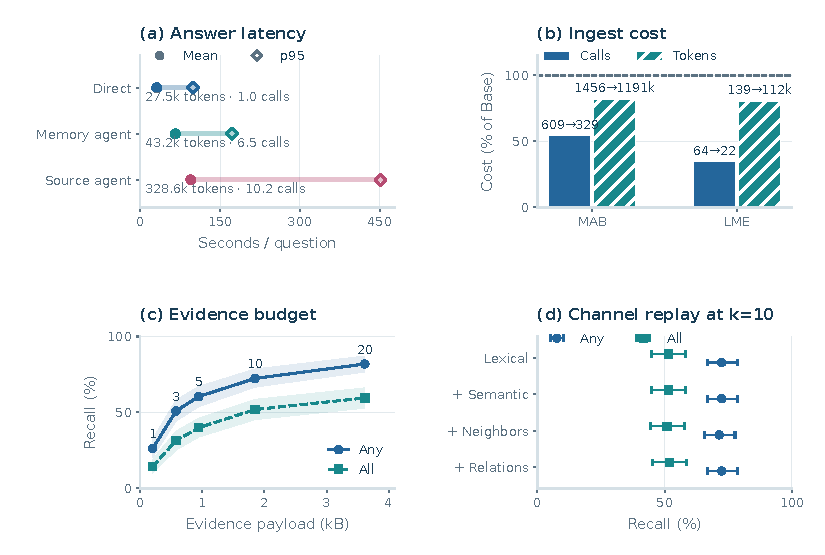
\includegraphics[width=\columnwidth]{figures/fig3_cost.pdf}
  \caption{冻结产物的运行点诊断（Align+ 引擎；面板 a 覆盖全部 1{,}074 题）。(a) 答案延迟的均值到 p95，标注 token 数与调用数；(b) 配对的 Base$\to$Align+ 入库成本；(c) 有效的固定排序检索预算前沿；(d) $k{=}10$ 处的仅源文档通道重放。}
  \label{fig:cost}
\end{figure}

\subsection{附加定量诊断}
\label{app:additional-diagnostics}

账本还包含类型级更新分数、一次受控的源扩展重放，以及 MEME 删除边界。图~\ref{fig:diagnostics} 报告这些量，并让样本量与开发集限制保持可见。

\begin{figure*}[t]
  \centering
  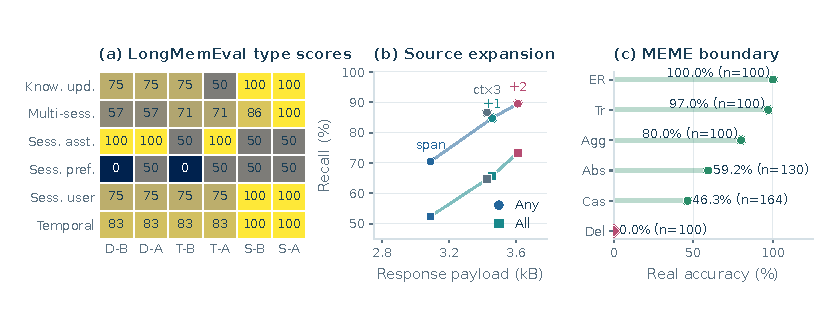
\includegraphics[width=\textwidth]{figures/figC_diagnostics.pdf}
  \caption{来自冻结账本的额外定量诊断。（a）配对 Base/Align+ 轨道的 LongMemEval 类型分数；这些方向性样本 $n{=}25/25/27$，以粗略百分比显示。（b）105 个历史错误案例上的源扩展召回对响应载荷；这是开发诊断，不是留出测试。（c）带任务特定分母的 MEME 真实任务准确率，暴露 0\% 的删除边界。}
  \label{fig:diagnostics}
\end{figure*}


\subsection{载体参照（BigCodeBench \citep{zhuo2024bigcodebench}、ALFWorld \citep{shridhar2021alfworld}）}
\label{app:carrier-anchors}

BigCodeBench：0.4859 完成率 / 0.2838 困难 pass@1（校准切分）。ALFWorld：0.9786 同分布 / 0.9851 异分布成功率。两者都是对记忆不敏感的智能体载体回归测试：它们锚定智能体载体能正确执行任务，而不与记忆基准横向比较。

\subsection{MAB 入库清单缺口}
\label{app:manifest-gaps}

Base 与 Align+ 的 MAB 入库运行共享 45 份文档的配对交集。在某一代中缺失清单的文档被排除在每文档效率比之外，因此效率比只在交集上计算（每文档调用 609$\to$329，$-46\%$）；token 比使用同一交集。题目级结果不受影响：全部 767 道配对题在两代中都对着冻结库运行，307 道扩展题只在 Align+ 引擎上运行，因此入库成本比仍定义在配对交集上。

\subsection{预算前沿}
\label{app:budget}

早期的一次 depth-10 对 depth-20 重放作为一项完整性发现被保留：其前缀不变量在全部 210 题上失败（\texttt{primary\_result\_invariant\_violations=210}），因此它不用于任何正面主张。修复后的设计对每个查询以最大深度只运行一次检索，并把固定的排序切到 $k\in\{1,3,5,10,20\}$；前缀单调性因此按构造成立（零违例），前沿从 $k{=}1$ 到 $k{=}20$ 单调上升，每个 $k$ 的百分位 bootstrap 置信区间从冻结的重放产物重新计算。

\subsection{X7 通道消融细节}

\begin{table*}[t]
\centering
\caption{X7 来源记录消融：210 题检查集上的离线检索重放。臂 1--4 构成干净的通道消融：只有 \texttt{enabled\_channels} 不同，因此任何召回差异都可归因于该通道集合。臂 5（引用核对智能体，开启检查）与臂 6（未被检索到的证据，放宽检查）复用臂 4 的五通道排序，与臂 4 检索一致；它们的区分列（问答准确率、无支撑答案率、平均证据 token）需要 LLM 智能体运行，尚待完成。引用检查流程已离线验证：开启检查时提交一个未浮现的对话轮会被拒绝；放宽检查时同一提交被接受（\texttt{plumbing\_ok}=true）。在部署的 MAB 运行中，检查按设计触发：\GateRejectStats{}。Bootstrap 置信区间：2{,}000 次重采样，95\%。}
\label{tab:provenance-ablation}
\small
\setlength{\tabcolsep}{3pt}
\begin{tabular}{llrrr}
\toprule
臂 & 通道(累加) & Recall-any@10 [95\% CI] & Recall-all@10 [95\% CI] & 平均字节@10 \\
\midrule
1 & raw-doc + episode-bm25 & 72.38 [66.67, 78.57] & 51.43 [44.76, 58.10] & 1833 \\
2 & + semantic-provenance & 72.38 [66.67, 78.57] & 51.43 [44.76, 58.10] & 1841 \\
3 & + graph-neighbor & 71.43 [65.70, 77.62] & 50.95 [44.29, 57.62] & 1845 \\
4 & + relation-evidence (full 5) & 72.38 [66.65, 78.57] & 51.90 [45.24, 58.58] & 1847 \\
\bottomrule
\end{tabular}
\end{table*}



\subsection{测试条件说明}

原始 LoCoMo token-F1 轨道含 1{,}986 题与五个类别。Mem0 兼容轨道含 1{,}540 题与四个类别。LongMemEval-S 含 500 题；整批写入后的配对运行使用 \cref{sec:setup} 所述的 $n{=}25/25/27$。MEME 的 100 个会话片段产生异质的任务数（所引运行中 ER/Agg/Tr/Del/Cas/Abs 的事后检查数为 100/100/100/100/164/130）。raw 分数与 real 分数不可互换。

\subsection{保留的完整性失败}

\cref{app:budget} 的深度重放报告 \texttt{primary\_result\_invariant\_violations=210} 且 \texttt{passed=false}。MEME 删除结果为 0\% 的 real 准确率。X7 通道消融是零结果，以等价界的形式报告而非丢弃。$\infty$Bench-Sum 的 $n{=}1$ 翻转直接使 Align+ Overall 损失 2.7 分（Base$\to$Align+ 净差距为 1.8 分），并在每处比较中披露。LongMemEval 上直接检索与工具辅助读取打平的结果虽然对记忆工具路径不利，仍予报告。这些记录保持可见，因为一篇可审计的记忆论文应当同时暴露失败与零结果的机制，而不只是成功的机制。

\subsection{外部比较协议}
\label{sec:published-baselines}

Mem0 原论文报告 LoCoMo 类别级 F1、BLEU-1 与一个二值 $J$：GPT-4o-mini 评审把每个答案标为 CORRECT 或 WRONG，得分即判定为 CORRECT 的百分比（10 次独立运行的均值$\pm$标准差）。Zep 原论文报告 DMR 与 LongMemEval，答题模型为 GPT-4o 系列。我们不在自己的协议下重跑这些系统，而是在下方逐字重印其已发表表格（表~\ref{tab:mem0-baselines}--\ref{tab:zep-longmemeval}）作为不同测试流程下的参考结果。因篇幅从正文表格中省略的 Mem0 确定性 token 重叠指标重印于表~\ref{tab:mem0-f1-bleu}。

\begin{table*}[t]
\centering
\small
\setlength{\tabcolsep}{2pt}
\renewcommand{\arraystretch}{1.12}
\begin{tabular*}{\textwidth}{@{\extracolsep{\fill}}>{\raggedright\arraybackslash}p{0.30\textwidth}>{\raggedright\arraybackslash}p{0.21\textwidth}>{\centering\arraybackslash}p{0.16\textwidth}>{\raggedright\arraybackslash}p{0.29\textwidth}@{}}
\toprule
基准 & 协议 & 分数 & 答题 / 评审 \\
\midrule
LongMemEval-S (500) & 抽样，$n{=}500$ & 84.60 & Qwen3.7-plus 作答；Qwen3.7-plus 评审 \\
LongMemEval，直接检索 & 配对，$n{=}25$ & 0.68 $\to$ 0.72 & Kimi-K3 作答 \\
LongMemEval，工具辅助读取 & 配对，$n{=}25$ & 0.68 $\to$ 0.72 & Kimi-K3 作答 \\
LongMemEval，原文读取 & 配对，$n{=}27$ & 0.889 $\to$ 0.926 & Kimi-K3；自评审 \\
LoCoMo-1540 & Mem0 $J$ 评分 & 95.19 & Kimi-K3；作答+评审；$n{=}1$ \\
LoCoMo-1540（同一批答案） & 交叉评审 & 94.22 & Qwen3.7-plus；一致率 98.51\% \\
\bottomrule
\end{tabular*}
\caption{其他基准在各自测试流程下的结果；每行列出答题模型和评审模型。LoCoMo 运行与 Mem0 已发表的 $J$ 有两处明示差异——单次运行对 10 次运行均值$\pm$标准差，以及作答/评审模型——并携带已披露的遗留指纹注意事项；这些条件同时列出，便于复核比较。LME 原文读取轨道多出的两题来自其会话证据规则；比较只在同一测试轨道内进行。}
\label{tab:protocol-other}
\end{table*}


\textbf{K3 替换行。}
\label{app:k3-substitution}
放入 Mem0 $J$ 列内的唯一一行 Deep-Dream $J$，是用 Mem0 原样的二值评分方式、以 Kimi-K3 同时替换 GPT-4o-mini 的答题与评审角色得到的——唯一的改动就是模型。同模型 K3 评审下得 95.19\%（S/M/O/T 为 97.38/93.62/80.21/95.33）；同一批 K3 答案经独立的 Qwen3.7-plus 交叉评审得 94.22\%（96.91/92.91/77.08/93.46；交叉评审一致率 98.51\%）。相对 Mem0 已发表 $J$ 的两处差异照例明示：单次运行而非 10 次运行均值$\pm$标准差；模型为 Kimi-K3 而非 GPT-4o-mini。我们额外披露一条完整性注意事项：该运行清单带有 \texttt{diagnostic\_override=\{kind:legacy-missing-runtime-code-fingerprint, formal\_claim\_allowed:false\}}，因为 1{,}540 行答案中有 1{,}529 行来自早于运行时代码指纹机制的遗留源运行（\texttt{legacy-source-run}）。答案本身未变（\texttt{answer\_rows\_unchanged=true}，答案 SHA-256 为 76af5772），且逐题 JSONL 在全部 2{,}063 行上都带 \texttt{runtime\_code\_sha256}（3 个不同哈希：2fa32774 覆盖 2{,}019 行、36b45933 覆盖 33 行、42afb1ac 覆盖 11 行），数据集 SHA-256（79fa87e9）与库快照（cf2e76b8）与 Qwen 作答运行相同，Mem0 二值评审提示词也相同（仓库 \texttt{mem0ai/memory-benchmarks}，commit 4b61c5d，模式 \texttt{unified-no-evidence-exact-direct}）。因此我们把 95.19\% 报告为诊断性交叉评审结果，而不是指纹完备的正式条目。

更严格的受控比较——冻结相同的答题模型、评审模型、提示词、温度、证据预算、数据集修订版本与 Graphiti/Zep 实现 commit——仍是通向共享榜单的唯一途径；但既然已发表数字被直接引用，它不再是投稿的硬性门槛。

\subsection{架构的信息论读法}
\label{app:info-theory}

本附录给论文的两条设计承诺一个形式化表述。每一条陈述要么是架构的结构性质（可对照 schema 与代码检查），要么是带显式假设的条件命题；没有一条提升 \cref{sec:ladder,sec:provenance-ablation} 的因果措辞纪律。

\subsubsection{写入时：渐进式实体对齐}

设不可变源流为 $S=D_1,\ldots,D_T$。每条抽取出的提及产生一个特征向量 $X_t$，包含名称与内容嵌入、属性以及关系端点共现。设 $Z$ 为潜在实体指派，$M_t=(F_t,O_t,G_t)$ 为 $t$ 条观测后的状态：概念族 $F_t$、只增观测库 $O_t$ 与关系图 $G_t$。观测从不被摘要替换；它始终保持与其精确源跨度的链接。

\begin{equation}
  \begin{aligned}
  O_{t+1}&=O_t\cup\{(X_{t+1},\mathrm{span}_{t+1})\},\\
  I(Z;O_{1:t+1})&=I(Z;O_{1:t})+
  I(Z;X_{t+1}\mid O_{1:t})\ge I(Z;O_{1:t}).
  \end{aligned}
  \label{eq:information-growth}
\end{equation}

第二个恒等式是只增流的记账事实：新观测可以增加关于身份的信息，而已有证据不会被丢弃。它解释了系统为何不必在首次提及时就解出实体链接。低置信度合并成为一个额外的族（过切分）；之后的观测可以通过重定向指针对族做合并，同时保留两边的观测集。过早的错误合并才是危险的错误，因为它把两个实体的证据污染进同一个检索位置。

\begin{proposition}[可修订性]
\label{prop:revisability}
在只增数据模型中，当前族划分的任何粗化都可以在之后由非破坏性合并实现，且不损失证据。若一个存储改为用滚动摘要 $\sigma$ 覆写实体，则由数据处理不等式有 $I(Z;\sigma)\le I(Z;O)$，且每当身份可判别的细节被丢弃时不等式严格。
\end{proposition}

\begin{proposition}[汇聚证据下的收敛]
\label{prop:convergence}
假设特征在给定实体身份时 i.i.d.，且两个不同实体 $e\ne e'$ 的输出分布 $P_e\ne P_{e'}$ 具有 Chernoff 信息 $C(P_e,P_{e'})>0$。对使用 $k$ 条汇聚观测的同/异实体检验，似然比误差满足 $\Pr[\mathrm{error}]\le\exp[-kC(P_e,P_{e'})]$ \citep{chernoff1952measure}。因此，一个在弱证据下被初始拆分的真实合并未被察觉的概率，随佐证证据指数下降。
\end{proposition}

这些假设是理想化的：真实窗口相关、抽取噪声重尾、同名异实体对的 $C$ 可能很小。因此该预测是定性的，而不是一个实测收敛速率。它与实现的批量处理和末尾复查一致——后者用更多汇聚上下文重测候选族。在配对引擎运行中，同名重复组从 340$\to$124（MAB）、482$\to$99（LME），每文档入库调用下降 46--65\%；这些是实测参考值，不是对 $C$ 的估计。关系边承担两个角色：端点共现在写入时帮助区分假设，所得的图在读取时提供额外路径。

\subsubsection{读取时：层级检索位置与渐进披露}

派生层是一个检索索引，而不是答案重构。设 $A_t(q)$ 把问题映射到概念族与关系邻域，$\rho$ 为选择打开哪些候选的智能体策略。所得的源上下文构成一条自适应链
\begin{equation}
  C_0(q)\subseteq C_1(q)\subseteq\cdots\subseteq S,\qquad
  a_{k+1}=\rho\bigl(q,M_t,C_{\le k},u_k\bigr),
  \label{eq:progressive-disclosure}
\end{equation}
其中 $u_k$ 是智能体的当前不确定性。概念搜索给出快速的宏观检索线索；族观测与关系边对其精化；最终读取返回确切的会话片段与跨度。这正是同一表示既支持自主探索、又支持读取原文答案的原因。

把重构失真定义为被引用文本与其声称代表的源文本之间的差异，把寻址损失定义为未能把相关源跨度放入 $C_k$。由于每条路径都把候选解析到逐字源跨度、且引用检查只接受当前回合浮现的跨度，重构失真按构造为零；全部残余损失都是寻址损失。摘要式记忆在写入时固定一个率--失真点，而 $\rho$ 逐查询选择阅读预算 \citep{shannon1959coding}。智能体可以在一次紧凑的概念查询后停止，也可以在不确定性仍高时披露更多邻域与源文件，而不改变证据的权威性。

\subsubsection{双速率分解与答案风险}
设 $A(q)$ 为派生派生图层输出的检索位置，$E_C$ 为候选集 $C$ 选出的精确源跨度。对答案相关变量 $Y$，链式法则给出
\begin{equation}
  I(Y;A,E_C\mid Q=q)=I(Y;A\mid Q=q)+I(Y;E_C\mid A,Q=q).
  \label{eq:appendix-two-rate}
\end{equation}
第一项是紧凑概念/关系检索位置提供的信息；第二项是打开源文本才获得的信息。纯摘要记忆把 $S$ 替换为信道输出 $\widetilde S=f(S)$，无法使 $I(Y;\widetilde S\mid Q)$ 超过 $I(Y;S\mid Q)$；Deep-Dream 则在寻址之后仍保持源信道可用。这是一种信息瓶颈解释，而不是“实现解决了该瓶颈变分问题”的主张 \citep{tishby2000information}。

为完整起见，设 $R_q$ 为相关源跨度被寻址这一事件，$V_q$ 为验证者在读取后正确作答这一事件。则
\begin{equation}
  \Pr[\widehat Y=Y\mid q]\ge \Pr[R_q\mid q]\Pr[V_q\mid R_q,q].
  \label{eq:appendix-answer-bound}
\end{equation}
派生图层主要影响检索位置召回，逐步读取原文影响条件验证。引用检查在其显式可达性契约下把引用来源错误的概率设为零；语义不相关仍在保证之外。该分解解释了为什么改进应当在需要多次提及、时序更新或事实整合的问题上最大，以及为什么仅图的离线召回变化不必预测完整的在线增益。

扩展样本上 Align+ 的实测运行点为（27.5k token，0.333）、（43.2k，0.400）与（328.6k，0.710）的 Overall；冻结在配对样本上的 Base 代复现了该次序（0.3025/0.3759/0.6695）。FC-MH 分数（2--4 对 67--70）显示了自适应源阅读在何处最重要。X7 在开发切片上把派生通道的离线检索贡献界定在 $\pm2.4$ 分以内；派生图层的在线价值是文档组选择与链接扩展，由原文读取智能体行使，而不会被该消融移除。

\begin{samepage}
\begin{proposition}[单侧寻址错误]
\label{prop:one-sided}
对任何派生图层状态，$A_t$ 中的错误可以改变哪些跨度进入 $C_k$，但不能改变被引用检查接纳的跨度的文本或溯源。因此派生图层错误造成的是覆盖缺失，而不是捏造的引用内容；该保证是被引用原文是否被打开，不是语义蕴含。
\end{proposition}
\end{samepage}

这套表述增加了数学结构，但没有提升阶梯的因果措辞：指数陈述是有条件的，重名计数是代理量，实测的阶梯仍是一个系统比较。

\begin{table*}[t]
\centering
\caption{LoCoMo 分类别 $J$（二值 CORRECT/WRONG 准确率，LLM 评审）。已发表行逐字复现自 \citet{chhikara2025mem0}（arXiv:2504.19413，表~1）：Mem0 报告 10 次运行的均值$\pm$标准差，答题与评审均为 GPT-4o-mini（标准差省略，全部 $\le$0.75）。\textbf{Deep-Dream} 应用固定在仓库提交 \texttt{4b61c5d} 的二值 $J$ 评分规则——该 2026 修订版评审提示的容差规则异于 2025 年论文的附录 A——以 Kimi-K3 同时作答与评审（单次运行）；$\dagger$ 行用独立的 Qwen3.7-plus 交叉评审评判同一批 K3 答案（交叉评审一致率 98.51\%）。相同的 841/282/96/321 题目群体（共 1{,}540 题，Mem0 兼容子集）。\emph{注意事项：}K3 作答运行被标记 \texttt{formal\_claim\_allowed=false}——1{,}529 条历史答案行早于运行时代码指纹（答案未变，sha 76af5772；逐条 JSONL 携带 \texttt{runtime\_code\_sha256}）；作为诊断性交叉评审结果报告，而非指纹完备的正式结果。确定性的 F1/BLEU-1 因篇幅省略（表~\ref{tab:mem0-f1-bleu}）。加权 $J$（由已发表分类均值按 841/282/96/321 题量重加权）：Mem0 $\approx$62.14，$Mem0^g$ $\approx$61.36；其论文表 2 另报 Overall $J=66.88$（Mem0）与 $68.44$（$Mem0^g$）。Deep-Dream 聚合 $J$：95.19\% / 94.22\%（$\dagger$）。表体为已发表数据的逐字复现，保留英文。}
\label{tab:mem0-baselines}
\footnotesize
\setlength{\tabcolsep}{5pt}
\begin{tabular}{lc}
\toprule
Method & $J$ (S/M/O/T) \\
\midrule
LoCoMo & --- / --- / --- / --- \\
ReadAgent & --- / --- / --- / --- \\
MemoryBank & --- / --- / --- / --- \\
MemGPT & --- / --- / --- / --- \\
A-Mem & --- / --- / --- / --- \\
A-Mem* & 39.79 / 18.85 / 54.05 / 49.91 \\
LangMem & 62.23 / 47.92 / 71.12 / 23.43 \\
Zep & 61.70 / 41.35 / 76.60 / 49.31 \\
OpenAI & 63.79 / 42.92 / 62.29 / 21.71 \\
Mem0 & 67.13 / 51.15 / 72.93 / 55.51 \\
$Mem0^g$ & 65.71 / 47.19 / 75.71 / 58.13 \\
\textbf{Deep-Dream} & 97.38 / 93.62 / 80.21 / 95.33 \\
\textbf{Deep-Dream}$^\dagger$ & 96.91 / 92.91 / 77.08 / 93.46 \\
\bottomrule
\end{tabular}
\end{table*}

\begin{table}[t]
\centering
\caption{已发表的深度记忆检索（DMR）基线，逐字复现自 \citet{rasmussen2025zep}（arXiv:2501.13956）。DMR 包含 500 段多会话对话（5 个会话、每会话 $\le$12 条消息），每段对话一道单跳事实检索题。Deep-Dream 目前未运行 DMR，因此本表仅作上下文参照。表体保留英文原文。}
\label{tab:zep-dmr}
\small
\begin{tabular}{llr}
\toprule
Method & Answerer & Accuracy \\
\midrule
Recursive Summarization & GPT-4-turbo & 35.3\% \\
Conversation Summaries & GPT-4-turbo & 78.6\% \\
MemGPT & GPT-4-turbo & 93.4\% \\
Full-conversation & GPT-4-turbo & 94.4\% \\
Zep & GPT-4-turbo & 94.8\% \\
Conversation Summaries & GPT-4o-mini & 88.0\% \\
Full-conversation & GPT-4o-mini & 98.0\% \\
Zep & GPT-4o-mini & 98.2\% \\
\bottomrule
\end{tabular}
\end{table}

\begin{table}[t]
\centering
\caption{LongMemEval 主要结果。已发表行（GPT-4o-mini / GPT-4o，全上下文 对 Zep）逐字复现自 \citet{rasmussen2025zep}（arXiv:2501.13956）。\textbf{Deep-Dream} 行使用 Qwen3.7-plus 同时作答与交叉评审——这是一个不同的协议；其准确率（84.6\%）被放在已发表数字旁边，而非共享榜单。Deep-Dream 的延迟/平均上下文未在已发表协议下测量（---）。六类别分解见表~\ref{tab:zep-longmemeval-cat}。表体保留英文原文。}
\label{tab:zep-longmemeval}
\footnotesize
\begin{tabular}{llrrl}
\toprule
Answerer & System & Accuracy & Latency (s) & Avg.\ context \\
\midrule
GPT-4o-mini & Full-context & 55.4\% & 31.30 & 115k \\
GPT-4o-mini & Zep & 63.8\% & 3.20 & 1.6k \\
GPT-4o & Full-context & 60.2\% & 28.90 & 115k \\
GPT-4o & Zep & 71.2\% & 2.58 & 1.6k \\
\textbf{Qwen3.7-plus} & \textbf{Deep-Dream} & \textbf{84.6\%} & --- & --- \\
\bottomrule
\end{tabular}
\end{table}

\begin{table*}[t]
\centering
\caption{LongMemEval 六类别分解（二值准确率，\%）。已发表的全上下文与 Zep 数值逐字复现自 \citet{rasmussen2025zep}（arXiv:2501.13956）；\textbf{Deep-Dream (Q.)} 行是 Qwen3.7-plus 作答+交叉评审在相同六个类别上的结果。答题/评审不同，因此这是粒度匹配的上下文参照，不是共享榜单。会话偏好（Sess.\ pref.）是所有系统最难的类别。表体保留英文原文。}
\label{tab:zep-longmemeval-cat}
\footnotesize
\setlength{\tabcolsep}{3.5pt}
\begin{tabular}{lcccccc}
\toprule
System & Sess.\ pref. & Sess.\ asst. & Temporal & Multi-sess. & Knowledge upd. & Sess.\ user \\
\midrule
Full-ctx (4o-mini) & 30.0 & 81.8 & 36.5 & 40.6 & 76.9 & 81.4 \\
Zep (4o-mini) & 53.3 & 75.0 & 54.1 & 47.4 & 74.4 & 92.9 \\
Full-ctx (4o) & 20.0 & 94.6 & 45.1 & 44.3 & 78.2 & 81.4 \\
Zep (4o) & 56.7 & 80.4 & 62.4 & 57.9 & 83.3 & 92.9 \\
\textbf{Deep-Dream (Q.)} & \textbf{53.3} & \textbf{100.0} & \textbf{84.2} & \textbf{74.4} & \textbf{91.0} & \textbf{98.6} \\
\bottomrule
\end{tabular}
\end{table*}

\input{figures/TABLE_mem0_f1_bleu_appendix_zh}
